\documentclass[10pt]{article}
\usepackage[spanish]{babel}
\usepackage[utf8]{inputenc}
\usepackage{graphicx}
\usepackage{amsmath,amsthm,amssymb}
\usepackage{amsfonts}
\usepackage{bbold}
\usepackage[margin=1in]{geometry}
\usepackage[export]{adjustbox}
\usepackage{grffile}
\usepackage{titling}
\usepackage{titlesec}
\usepackage{mdwlist}
\usepackage{float}
\usepackage{fancyhdr}
\usepackage{hyperref}
\usepackage{mathtools}
\usepackage[sort&compress]{natbib}
\usepackage[ruled,vlined]{algorithm2e}
\usepackage{multirow}
\usepackage[T1]{fontenc}
\usepackage{listings}
\lstset{upquote=true}

\selectlanguage{spanish}

% \pagecolor{black}
% \color{white}

\DeclareTextCommandDefault{\textregistered}{\textcircled{ \check@mathfonts\fontsize\sf@size\z@\math@fontsfalse\selectfont R}}

\newcommand{\mybreak}{%
  \par
  \nointerlineskip
  \cleaders\vbox to 5ex{%
    \vss
    \hbox to \textwidth{\hss\vrule width 1\textwidth height 0.2pt depth 0.2pt\hss}
    \vss
  }\vskip5ex
}

\renewcommand{\headrulewidth}{0pt}

\renewcommand\maketitlehooka{
\vspace{-2cm}
\noindent
\begin{minipage}{0.1\textwidth}

\includegraphics[width=\linewidth]{Logo.png}
\end{minipage}
\begin{minipage}{0.8\textwidth}\raggedright
\ \textbf{Facultad de Ingeniería}\\
\ \textbf{Mastering ML: Tiny and Simple - Laboratorio Nube - Equipo Optimos}\\
\ PROFESORES: Elkin Garcia, Juan F. Perez, Rafael Martínez
\end{minipage}
\mybreak
}

\begin{document}
\title{Laboratorio Nube}
\date{}
\author{}
\maketitle
\vspace{-17ex}
\begin{table}[h]
\begin{center}
	\begin{tabular}{c c c c}
		\textbf{Apellidos} & \textbf{Nombres} & \textbf{Código} & \textbf{Login}\\
		\hline
		Mantilla Redondo & Alejandro & 201711304 & a.mantillar \\
		Manrique Moreno & Andrés & 201821413 & af.manrique \\
		\hline
	\end{tabular}
\end{center}
\label{tab:Nombres}
\end{table}

\section*{Equipo}

Somos Andrés y Alejandro, un equipo de investigadores en \textit{Machine Learning} dedicado al desarrollo de modelos predictivos de punta y a su despliegue en soluciones tecnológicas tipo \textit{edge computing} y en sistemas embebidos.

\section{Cuenta AWS}

Nosotros ya contamos con una cuenta AWS, por lo cual no hizo falta utilizar la cuenta temporal.

\section{Lanzar y conectarse a una instancia que actuará como dispositivo}

Creamos en AWS una instancia EC2 con las siguientes características:

\begin{itemize}
    \item \textbf{Nombre:} Optimos\_VM\_Instance
    \item \textbf{OS:} Amazon Linux
    \item \textbf{Tipo de instancia:} t2.micro
\end{itemize}

En la consola EC2 se puede ver la instancia creada corriendo (figura \ref{fig:INSTANCIA_EC2_CORRIENDO}).

\begin{figure}[H]
    \centering
    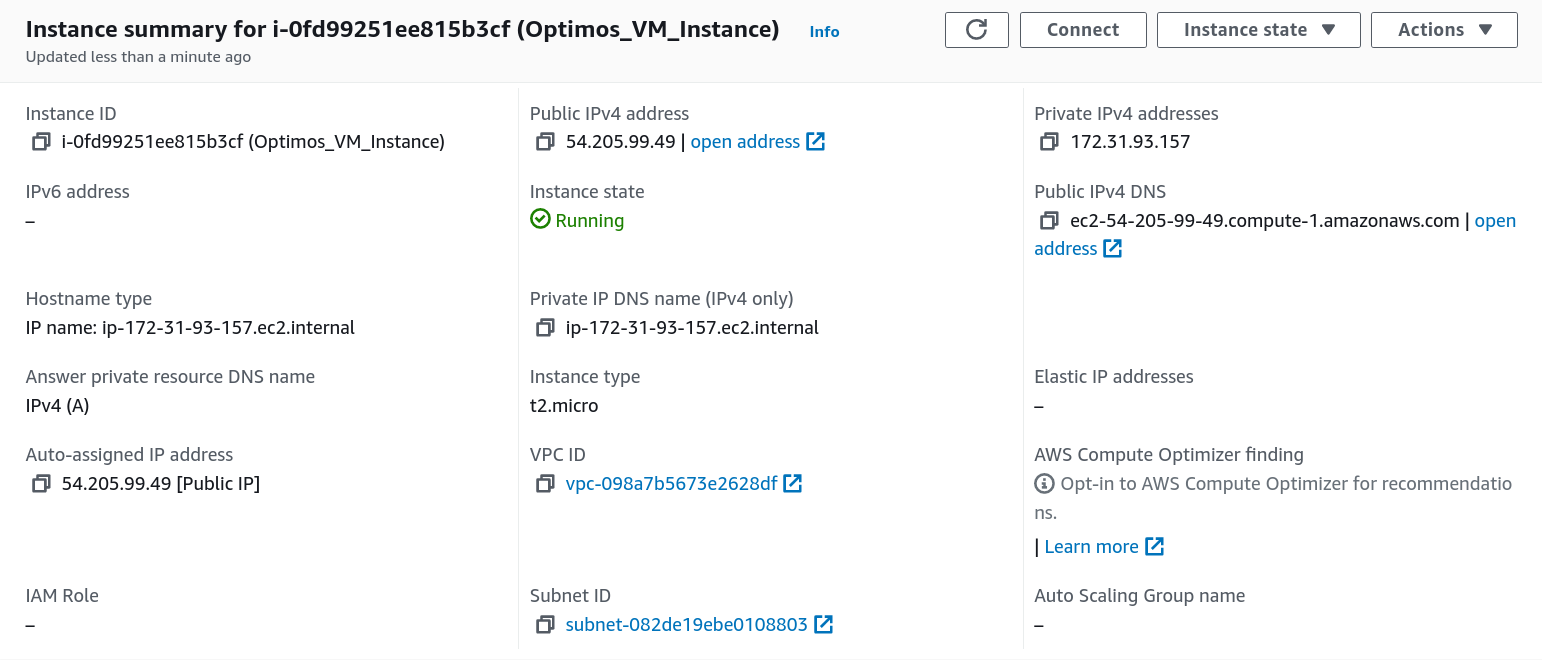
\includegraphics[width=0.8\textwidth]{Images/Running_instance_details.png}
    \caption{Instancia EC2 corriendo desde la consola de AWS.}
    \label{fig:INSTANCIA_EC2_CORRIENDO}
\end{figure}

Desde un computador local nos conectamos a la instancia EC2 remota por medio del protocolo SSH, como se ve en la figura \ref{fig:CONEXION_SSH}.

\begin{figure}[H]
    \centering
    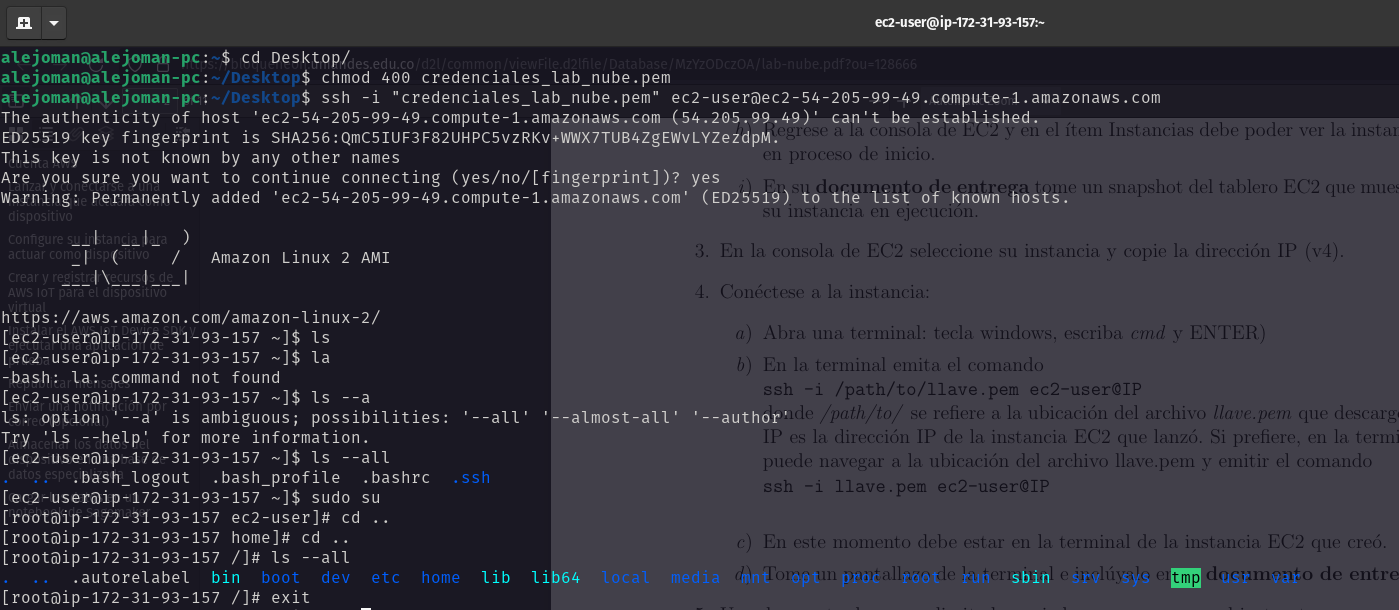
\includegraphics[width=0.9\textwidth]{Images/Instance_ssh_terminal.png}
    \caption{Conexión a instancia EC2 por SSH.}
    \label{fig:CONEXION_SSH}
\end{figure}

\section{Configure su instancia para actuar como dispositivo}

Configuramos la instancia de EC2 a una clave de acceso de la cuenta de AWS, lo que habilita un \textit{endpoint} con la dirección de la figura \ref{fig:json_endpoint}.

\begin{lstlisting}
{
    "endpointAddress": "a1b6n1ckf4d8zb-ats.iot.us-east-1.amazonaws.com"
}
\end{lstlisting}

\begin{figure}[H]
    \centering
    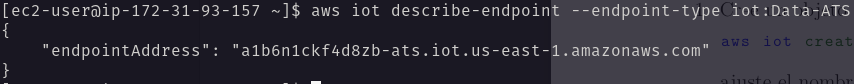
\includegraphics[width=0.8\textwidth]{Images/Endpoint_json_terminal.png}
    \caption{JSON con dirección de \textit{endpoint}.}
    \label{fig:json_endpoint}
\end{figure}

\section{Crear y registrar recursos de AWS IoT para el dispositivo virtual}

Procedemos a crear un recurso o \textit{thing} de AWS IoT en la instancia EC2. El nombre del recurso es \texttt{Optimos\_IOT\_thing} y sus atributos pueden verse en las figuras \ref{fig:Atributos_objeto_AWS_IoT} y \ref{fig:AWS_IoT_core_thing}. Ingresamos la respuesta JSON a continuación:

\begin{lstlisting}
{
    "thingArn": "arn:aws:iot:us-east-1:796184077497:thing/Optimos_IOT_thing",
    "thingName": "Optimos_IOT_thing",
    "thingId": "78b92fcf-0d28-4341-a03c-65407865bc7e"
}
\end{lstlisting}

\begin{figure}[H]
    \centering
    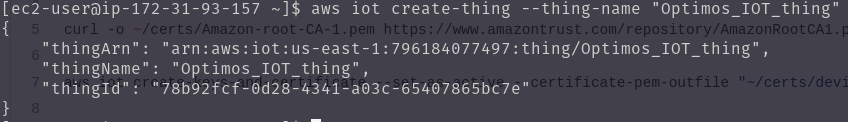
\includegraphics[width=0.8\textwidth]{Images/IOT_object_JSON_terminal.png}
    \caption{Atributos del recurso AWS IoT en formato JSON en la terminal.}
    \label{fig:Atributos_objeto_AWS_IoT}
\end{figure}

\begin{figure}[H]
    \centering
    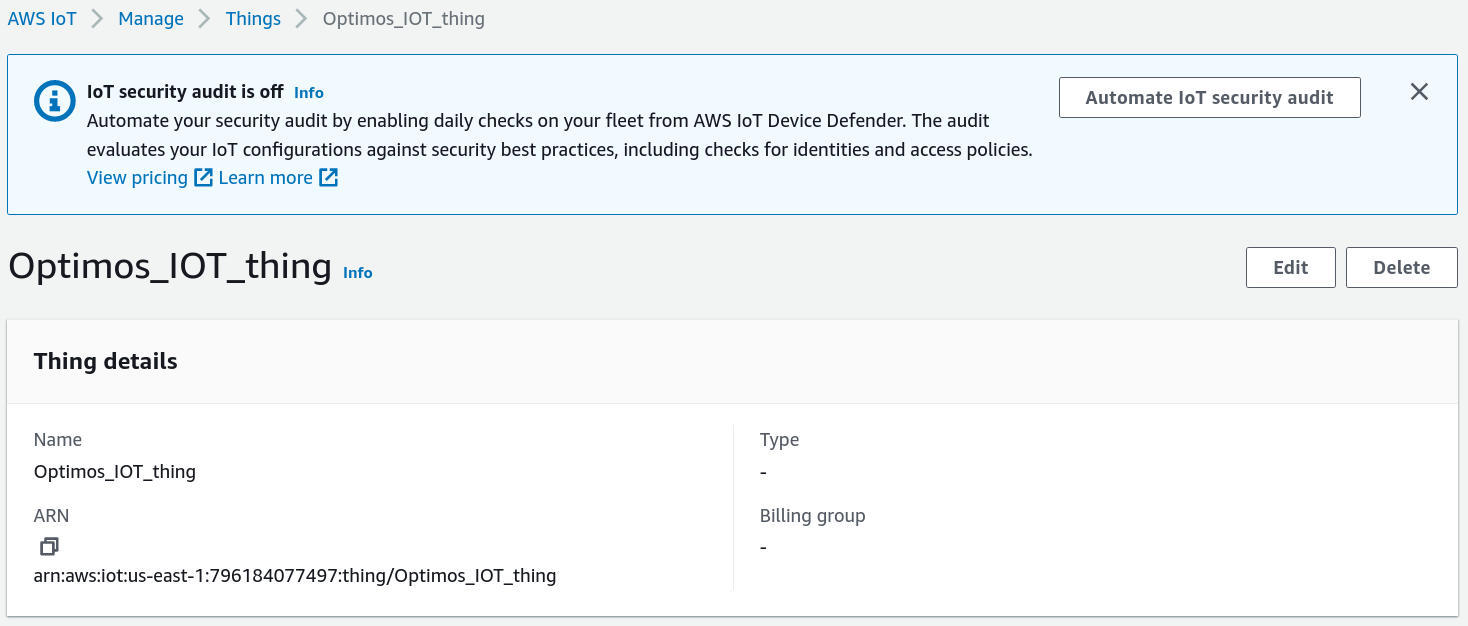
\includegraphics[width=0.8\textwidth]{Images/AWS_console_IOT_object.png}
    \caption{Recurso visible desde IoT Core.}
    \label{fig:AWS_IoT_core_thing}
\end{figure}

Creamos ahora un certificado para autenticar la identidad del dispositivo. El certificado ARN (Amazon Resource Number) obtenido lo obtuvimos del JSON en la figura \ref{fig:ARNcertificate}.

\begin{lstlisting}
{
    "certificateArn": "arn:aws:iot:us-east-1:796184077497:cert/15165fb098544f7
7f11500e850087457e60f770aee1aa0ffd0a3ee70aea4d57e",
    ...
}
\end{lstlisting}

\begin{figure}[H]
    \centering
    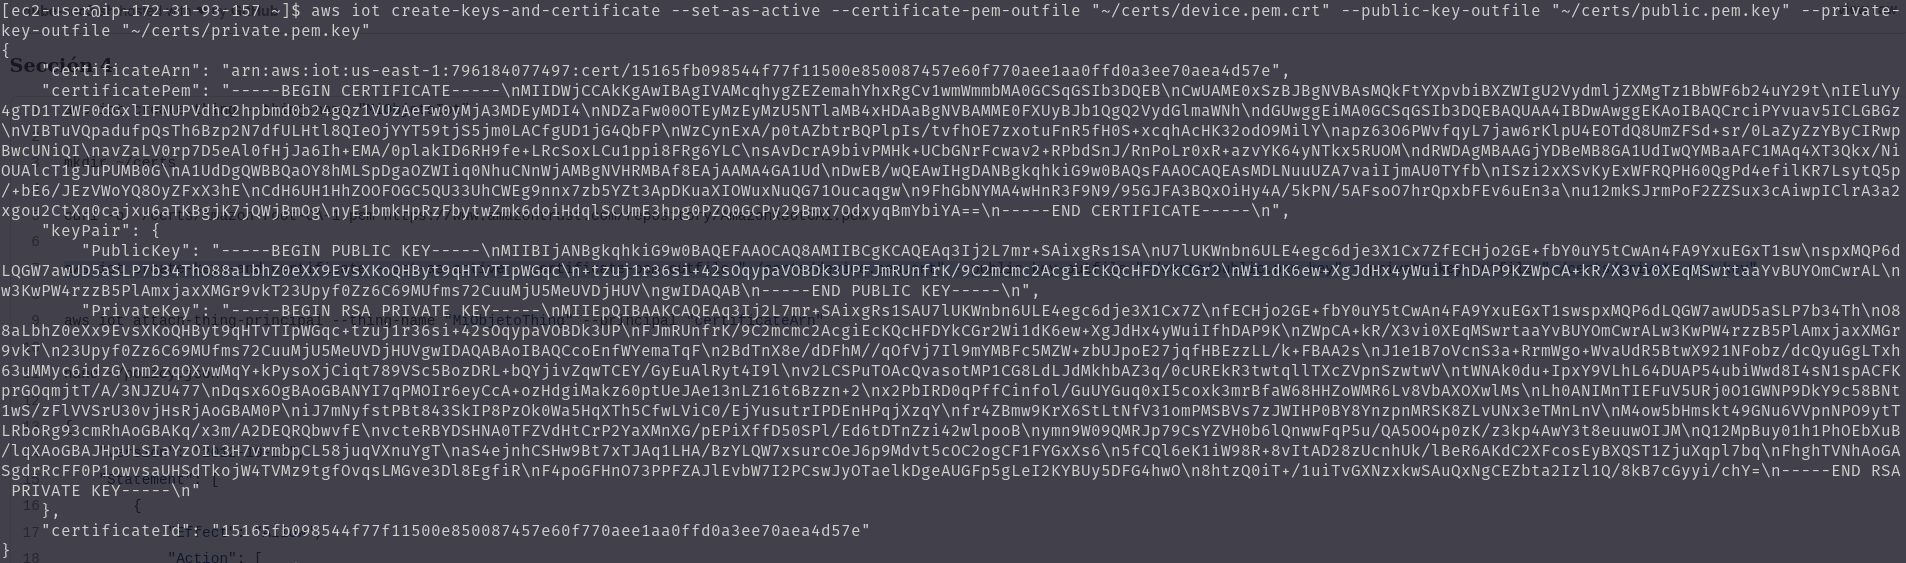
\includegraphics[width=\textwidth]{Images/ARN_JSON_terminal.png}
    \caption{Certificado ARN y otros atributos obtenidos en formato JSON.}
    \label{fig:ARNcertificate}
\end{figure}

En un nuevo archivo, \texttt{policy.json}, describimos una política para habilitar las acciones de publicar, suscribirse, recibir y conectarse. Estas operaciones son solo autorizadas para los recursos (en este caso IoT) que tengan el certificado adjunto. Esto es esencial para que el esquema de comunicaciones funcione apropiadamente ya que el recurso debe poder publicar y recibir mensajes, además de conectarse y suscribirse a otros dispositivos o tópicos.

\section{Instalar el AWS IoT Device SDK y ejecutar una aplicación de prueba}

Nuevamente, nuestra instancia de EC2 cuenta con el \textit{endpoint} de la figura \ref{fig:json_endpoint}.

Clonamos el repositorio, AWS IoT Device SDK, para publicar datos a un tópico. Ejecutamos la aplicación con el siguiente comando:

\begin{lstlisting}
node dist/index.js --topic topic_1 --ca_file ~/certs/Amazon-root-CA-1.pem --ce
rt ~/certs/device.pem.crt --key ~/certs/private.pem.key --endpoint a1b6n1ckf4d
8zb-ats.iot.us-east-1.amazonaws.com
\end{lstlisting}

Este comando subscribe a la máquina a un tópico al que puede publicar y del que puede recibir mensajes. En otras palabras, todo el proceso de autenticación realizado previamente permite en este punto poder publicar datos. Vemos, como \textit{logs} de la ejecución, los mensajes enviados al tópico (figura \ref{fig:mensajes_de_node_al_topico_terminal}) y los mismos mensajes desde la consola de AWS, por el cliente de MQTT (figura \ref{fig:mensajes_de_node_al_topico_MQTT}).

\begin{figure}[H]
    \centering
    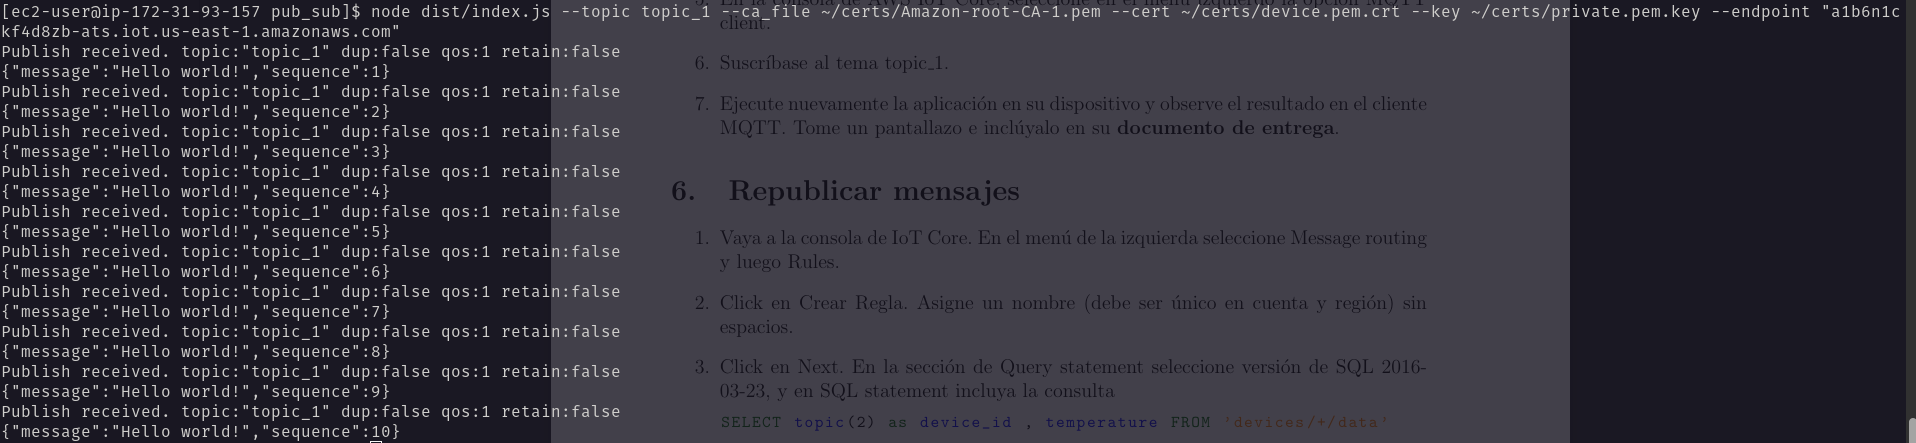
\includegraphics[width=1\textwidth]{Images/JSON_app_response_terminal.png}
    \caption{Mensajes publicados al tópico, \texttt{topico\_1}, por la aplicación, vistos desde la sesión SSH.}
    \label{fig:mensajes_de_node_al_topico_terminal}
\end{figure}

\begin{figure}[H]
    \centering
    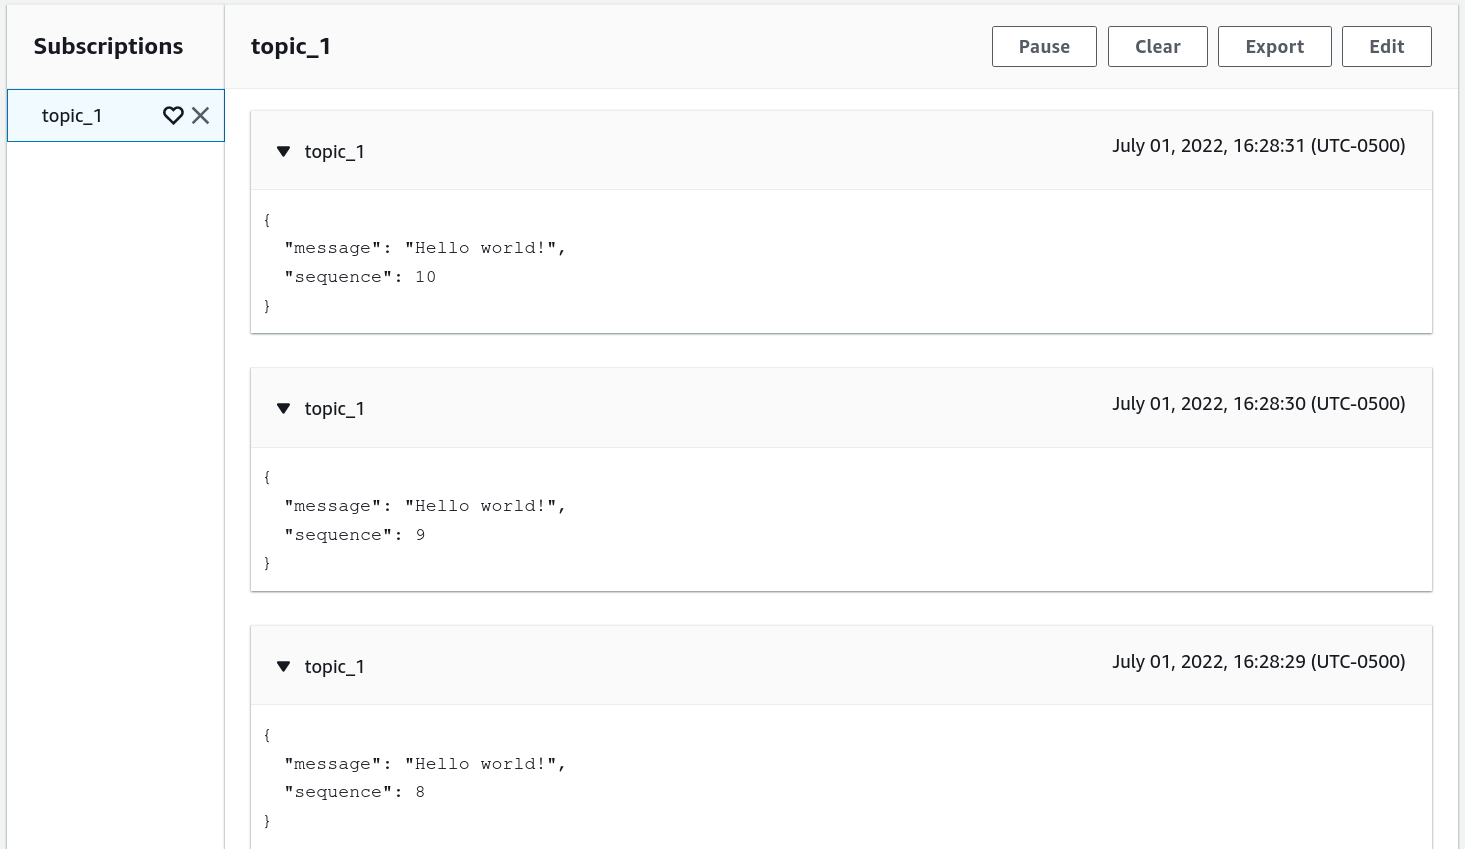
\includegraphics[width=0.8\textwidth]{Images/AWS_console_topic_1_subscription.png}
    \caption{Mensajes publicados al tópico, \texttt{topico\_1}, por la aplicación, vistos desde el cliente MQTT.}
    \label{fig:mensajes_de_node_al_topico_MQTT}
\end{figure}

\section{Republicar mensajes}

Añadimos una regle de reruteo de mesnajes con el siguiente \textit{query}.

\begin{lstlisting}
SELECT topic(2) as device_id , temperature FROM 'devices/+/data'
\end{lstlisting}

Este \textit{query} nos permite recuperar el ID del dispositivo desde el que se mandan los mensajes y el valor del campo \texttt{temperatura}, ya que coincide el \texttt{+} con cualquier dígito. Se capturan entonces los mensajes enviados a cualquier tópico de la forma \texttt{devices/<int>/data} y se vuelven a publicar al tópico \texttt{devices/data/temp}.

Identificamos cinco reglas adicionales que permiten redirigir los mensajes:

\begin{itemize}
    \item \textbf{Lambda:} envía el mensaje del tópico a una función Lambda, también implementada en AWS.
    \item \textbf{Salesforce IoT:} envía el mensaje devices/data/temp a un \textit{input stream} de Salesforce. 
    \item \textbf{HTTPS endpoint:} envía el mensaje del tópico a un HTTPS \textit{endpoint}.
    \item \textbf{S3 bucket:} envía el mensaje del tópico a a un S3 bucket (servicio de almacenamiento).
    \item \textbf{DynamoDB:} envía el mensaje del tópico a una tabla de DynamoDB (servicio de almacenamiento).
\end{itemize}

Ahora que estamos suscritos al tópico, \texttt{topico\_1}, validamos que en efecto se redirigen los mensajes de los dispositivos que cumplen con el patrón descrito (figura \ref{fig:mensajes_redirigidos_de_otros_topicos}).

\begin{figure}[H]
    \centering
    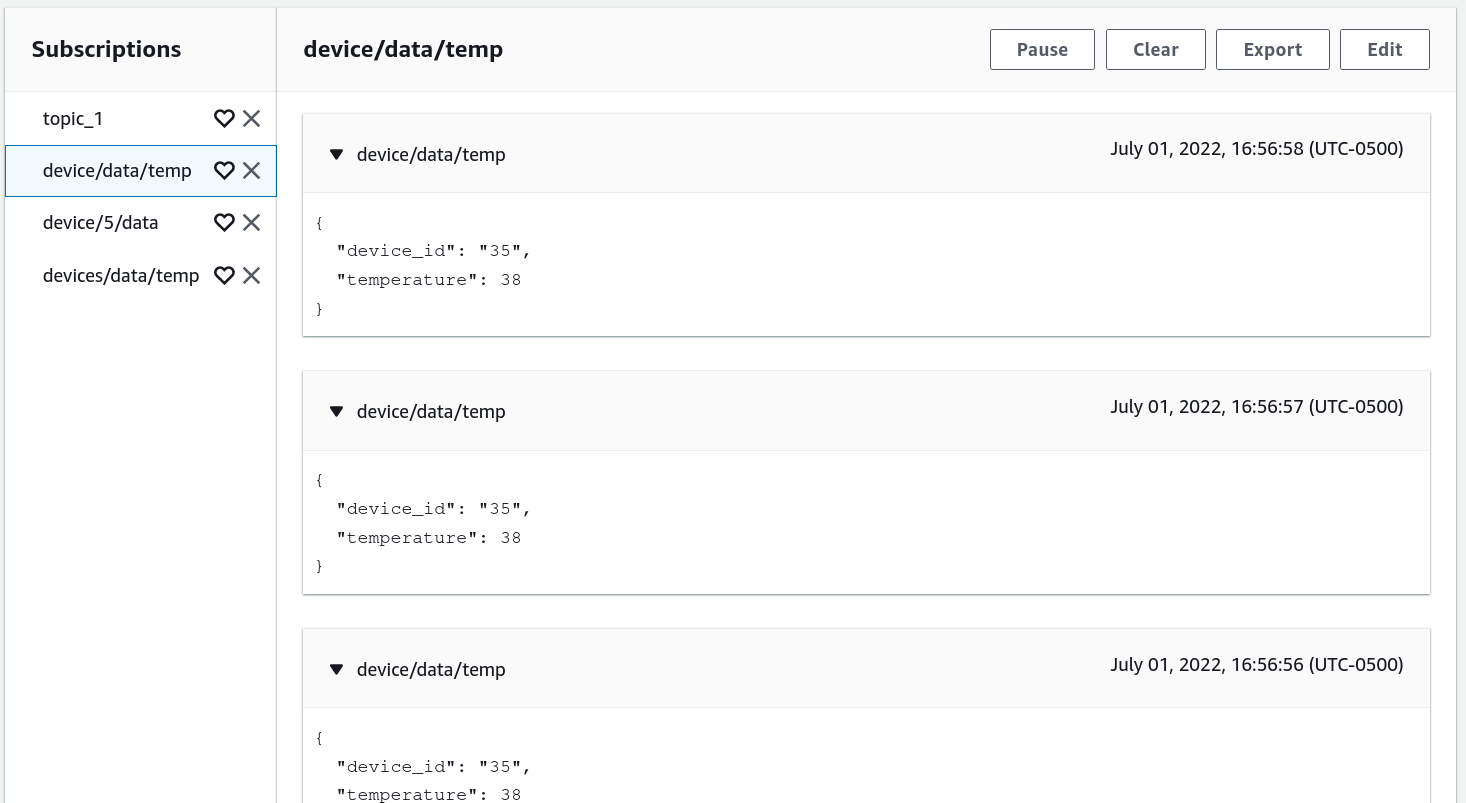
\includegraphics[width=0.8\textwidth]{Images/AWS_console_temperature_message_rceived.png}
    \caption{Mensajes con campos \texttt{device\_id} y \texttt{temperature}, redirigidos de otros tópicos.}
    \label{fig:mensajes_redirigidos_de_otros_topicos}
\end{figure}

Enviamos mensajes personalizados desde la sesión SSH y desde el cliente MQTT para validar que estén siendo redirigidos al tópico indicado.

\begin{figure}[H]
    \centering
    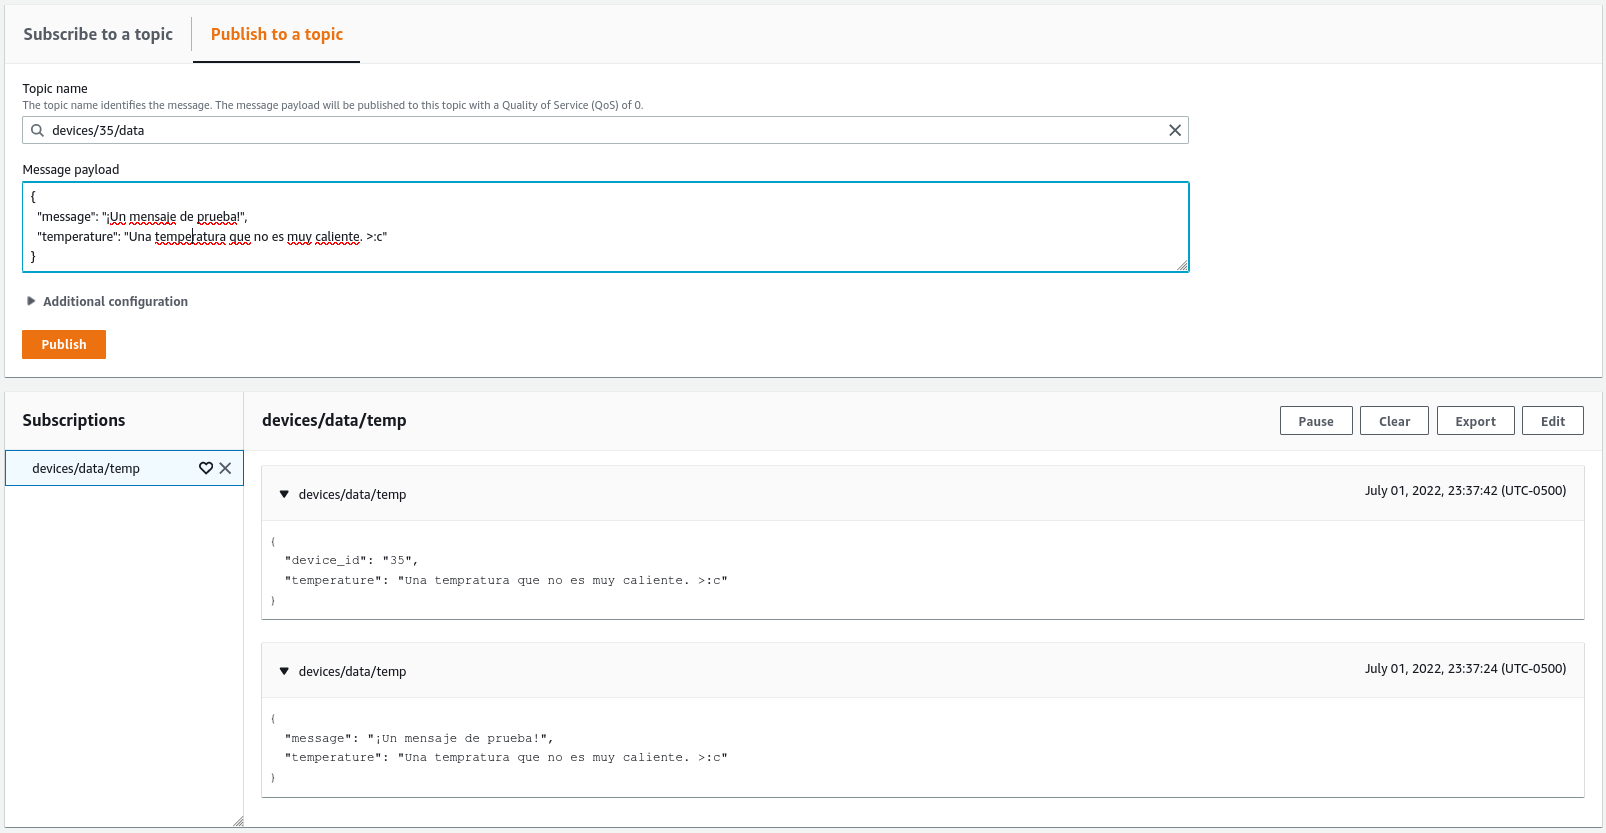
\includegraphics[width=0.8\textwidth]{Images/AWS_consola_mensaje_propio.png}
    \caption{Mensajes personalizados, redirigidos de otros tópicos.}
    \label{fig:mensajes_personalizados_redirigidos_de_otros_topicos}
\end{figure}

%#######################

\section{Enviar una notificación por correo (opcional)}

Reconocemos que para crear un tópico debemos escoger entre los tipos FIFO y Standard. Las características principales de FIFO es que da garantía de que los mensajes no se envían en desorden, y que se envía exactamente un mensaje. Estas restricciones no permiten tanto \textit{throoughput} y obliga a usar el protocolo SQS, a diferencia de Standard que relaja estas restricciones para permitir más \textit{throughput} y distintos protocolos de comunicación. En este segundo caso, los mensajes pueden llegar a repetirse y los mensajes pueden llegar en desorden, aunque se hace un esfuerzo por enviarlos según se acumulan en la fila.

Confirmamos la suscripción a los mensajes por correo siguiendo el enlace según la figura \ref{fig:suscripcion_correo}.

\begin{figure}[H]
    \centering
    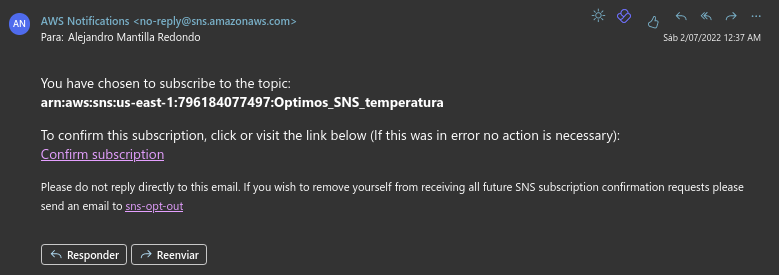
\includegraphics[width=0.8\textwidth]{Images/Correo_confirmacion_suscripcion.png}
    \caption{Mensaje de confirmación de suscripción a mensajes por correo.}
    \label{fig:suscripcion_correo}
\end{figure}

Damos clic desde la consola de AWS y publicamos un mensaje de prueba para validar que se satisface la suscripción. La figura \ref{fig:mensaje_prueba_correo} muestra que, en efecto, el correo llega exitosamente.

\begin{figure}[H]
    \centering
    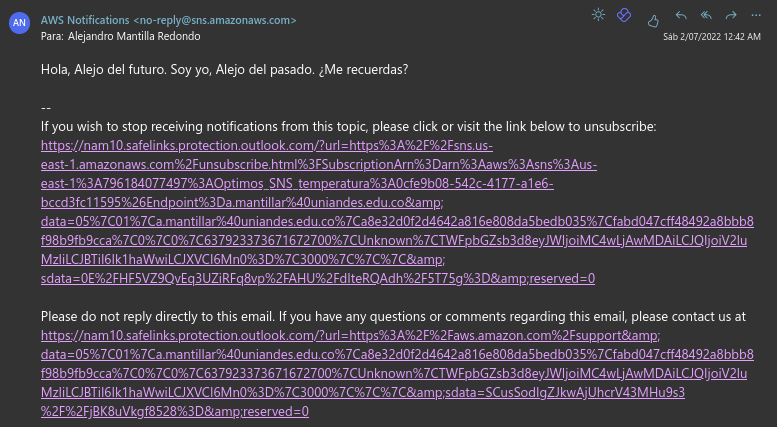
\includegraphics[width=0.8\textwidth]{Images/Mensaje_prueba_correo.png}
    \caption{Mensaje por correo de prueba.}
    \label{fig:mensaje_prueba_correo}
\end{figure}

Editamos el código del archivo \texttt{index.js} para que genere números aleatorios de temperatura en los mensajes, como podemos ver en el código a continuación.

\begin{lstlisting}
const msg = {
	message: argv.message,
	temperature: 15 + Math.floor(Math.random() * 20),
	humidity: 75,
	sequence: op_idx + 1,
	device_id: 3,
};
\end{lstlisting}

Este código produce un valor aleatorio entre 0 y 1, lo multiplica por 20, lo aproxima al entero inferior y le suma 15. El resultado es un número aleatorio entre 15 y 34.

Probamos enviar mensajes desde MQTT y desde SSH a nuestro correo por medio de las reglas que redirigen a SNS y confirmamos que llegan de manera apropiada (figuras \ref{fig:mensaje_redirigido_de_MQTT_a_correo} y \ref{fig:mensaje_redirigido_de_SSH_a_correo}).

\begin{figure}[H]
    \centering
    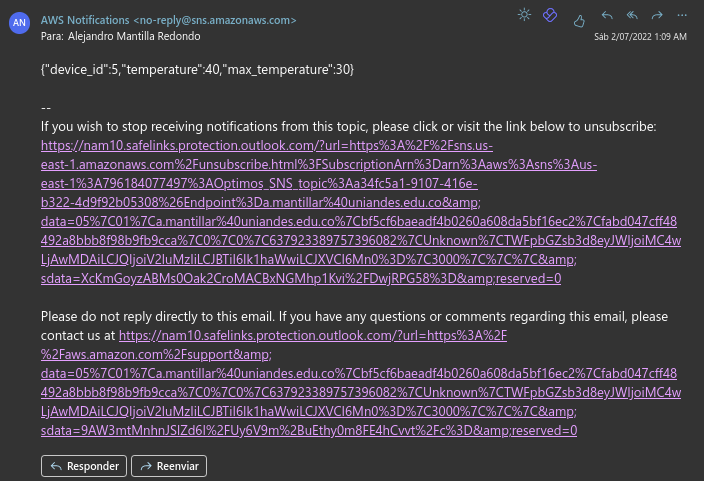
\includegraphics[width=0.8\textwidth]{Images/Mensaje_redirigido_de_MQTT_a_correo.png}
    \caption{Mensaje redirigido de MQTT a correo.}
    \label{fig:mensaje_redirigido_de_MQTT_a_correo}
\end{figure}

\begin{figure}[H]
    \centering
    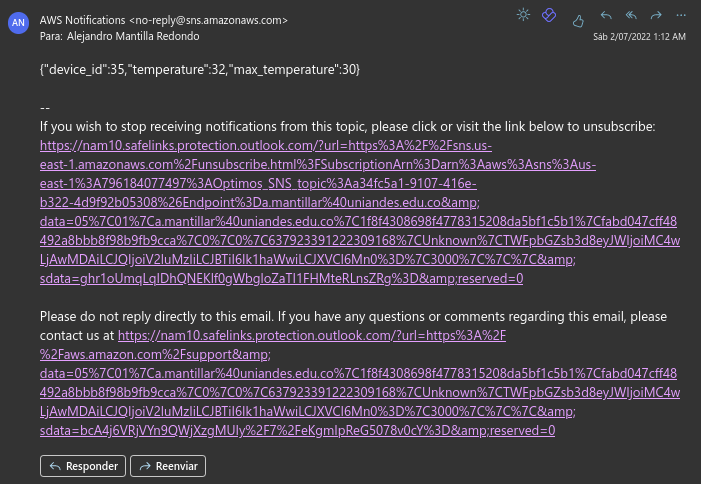
\includegraphics[width=0.8\textwidth]{Images/Mensaje_redirigido_de_SSH_a_SNS.png}
    \caption{Mensaje redirigido de aplicación en SSH a correo.}
    \label{fig:mensaje_redirigido_de_SSH_a_correo}
\end{figure}



%###################

\section{Almacenar los datos del dispositivo en una base de datos especializada}

Creamos ahora un \textit{Database} en Amazon Timestream. Tenemos dos campos a diligenciar: por un lado, permitir un \textit{data retention} de un día; por el otro, poner 7 días para retención magnética. La diferencia consiste en el tiempo en cada capa de almacenamiento, la velocidad de transferencias y en el costo de dicho almacenamiento. El almacenamiento estándar es veloz y costoso, de manera que es preferible para datos que deben leerse y escribirse con frecuencia en aplicaciones demandantes. El almacenamiento magnético es lento pero económico y sirve para almacenar datos accedidos con menos frecuencia o como respaldo, lo que lo hace una solución viable a más largo plazo.

Al crear una nueva regla para rutear los mensajes de los devices a una base de datos en Timestream, declaramos el siguiente \textit{query}:

\begin{lstlisting}
SELECT temperature FROM "devices/+/data"
\end{lstlisting}

Este \textit{query} recupera únicamente el campo de temperatura del mensaje. Validamos que nuestra regla está agregando mensajes nuevos a la tabla creada, según las figuras \ref{fig:query1} y \ref{fig:query2}.

\begin{figure}[H]
    \centering
    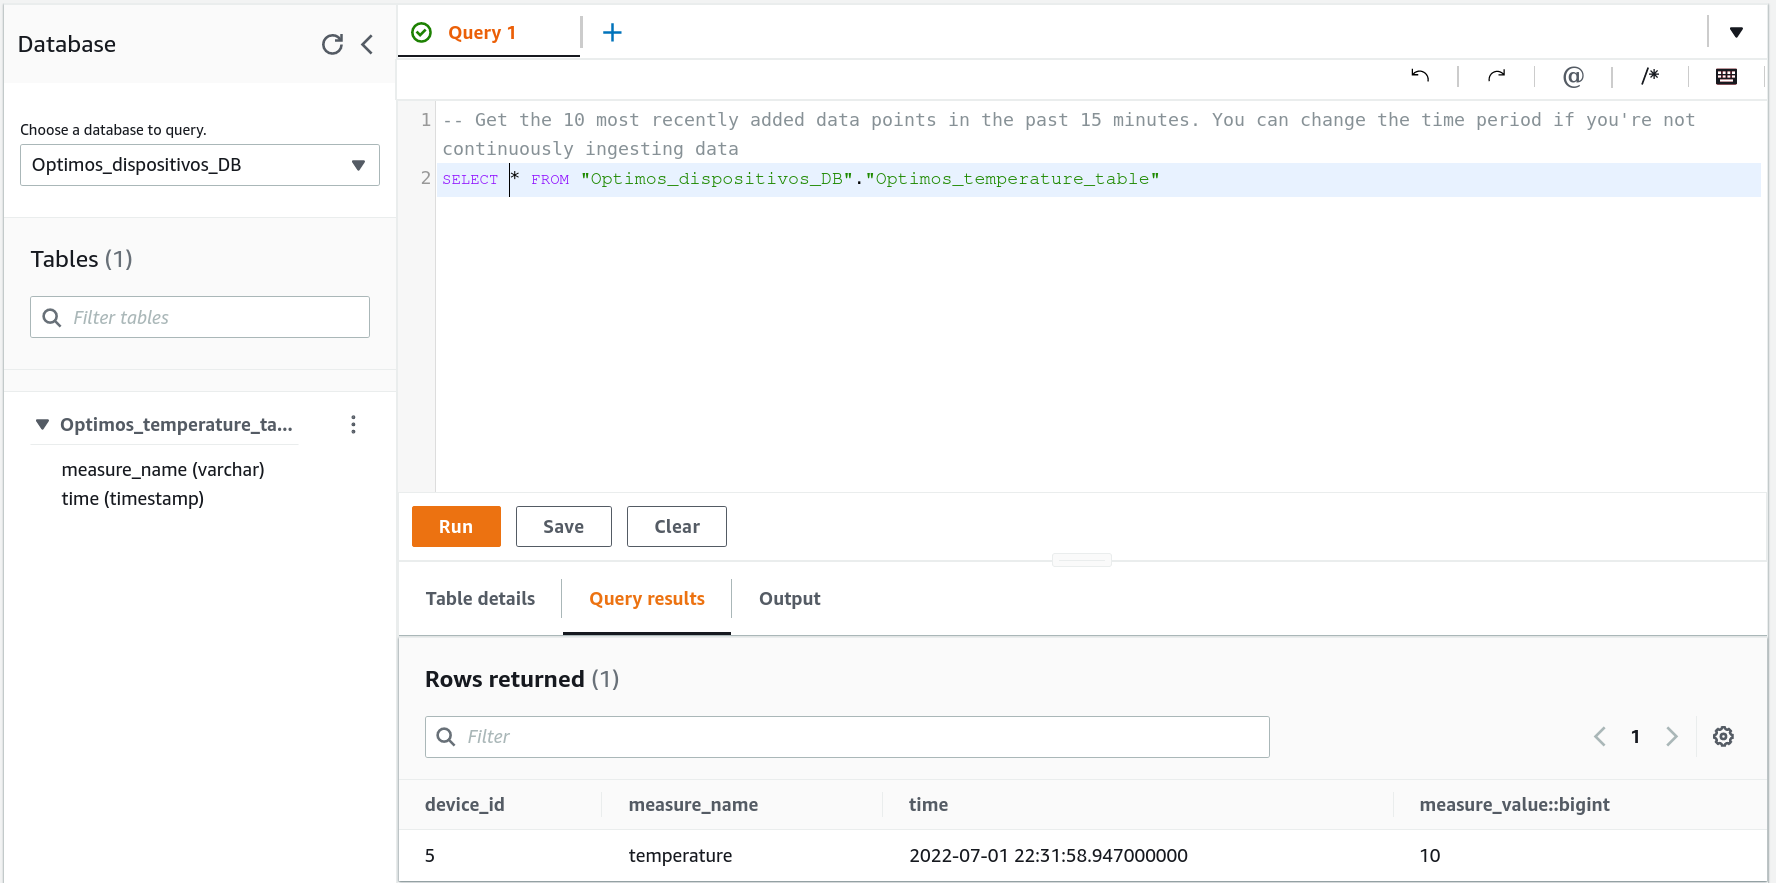
\includegraphics[width=0.8\textwidth]{Images/AWS_console_DB_query.png}
    \caption{Resultados del \textit{query} sobre la tabla desde Timestream, antes de agregar nuevos mensajes.}
    \label{fig:query1}
\end{figure}

\begin{figure}[H]
    \centering
    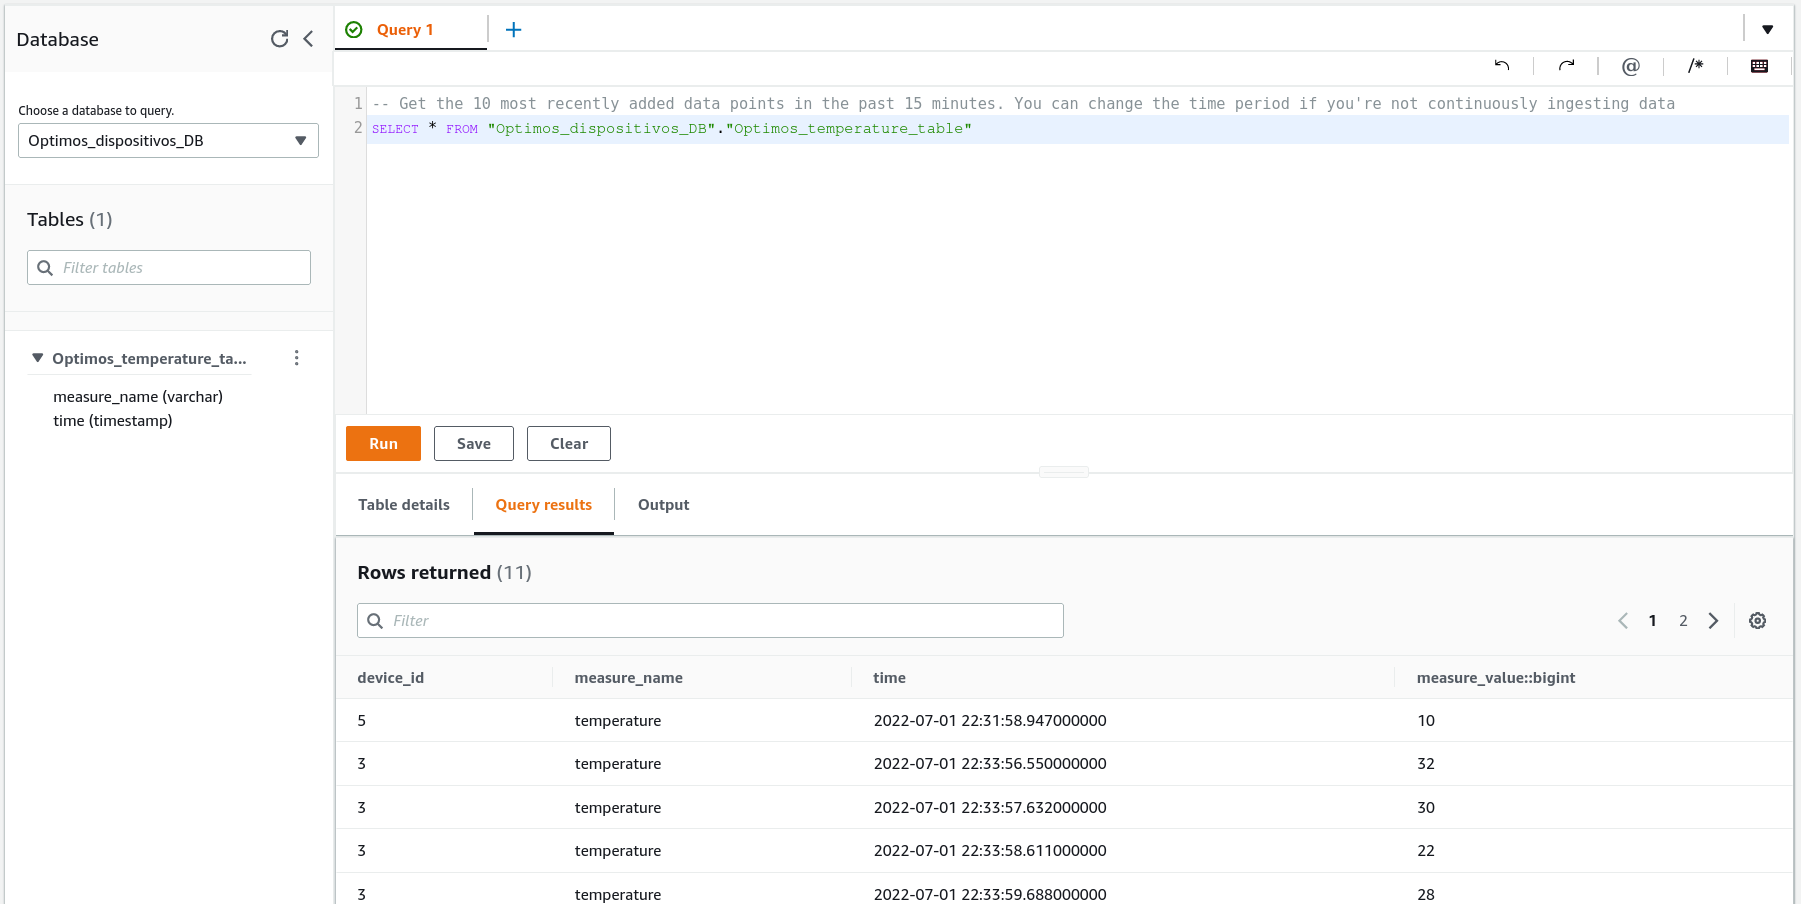
\includegraphics[width=0.8\textwidth]{Images/AWS_console_query_after_from_device.png}
    \caption{Resultados del \textit{query} sobre la tabla desde Timestream, luego de agregar nuevos mensajes.}
    \label{fig:query2}
\end{figure}

\section{Cargar los datos en un notebook de Sagemaker}

Usamos el servicio de Amazon Sagemaker para crear una instancia de Jupyter Notebook. Desde Jupyter, hacemos un query a la tabla de Timestream con la siguiente instrución:

\begin{center}
wr.timestream.query(
    'SELECT device\_id, time, measure\_value::bigint FROM "dispositivos\_temperatura"."temperatura" ORDER BY time DESC'
\end{center}

Este comando genera un problema de permisos ya que, por defecto, Amazon Sagemaker no tiene acceso a la base de datos en Timestream. Así, al darle los permisos se obtuvieron los resultados de la figura \ref{fig:sagemaker}.

\begin{figure}[H]
    \centering
    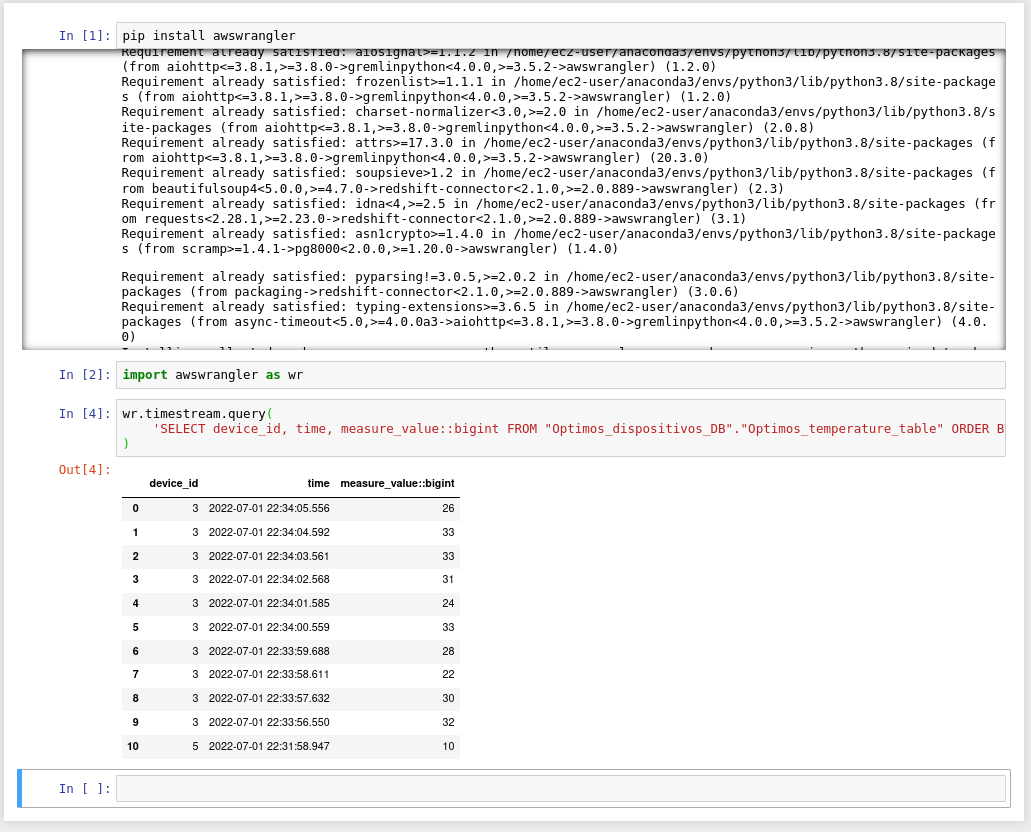
\includegraphics[width=0.8\textwidth]{Images/Jupyter_succesful_query.png}
    \caption{Tabla vista desde Jupyter en Sagemaker}
    \label{fig:sagemaker}
\end{figure}


%Bibliografía
%\clearpage 
%\bibliographystyle{plain}
%\bibliography{Biblio}
%Fin bibliografía

\end{document}